\documentclass[letterpaper, 10pt, onecolumn, draftclsnofoot]{IEEEtran}
\usepackage{enumitem}
\usepackage{geometry}
\usepackage{tabularx}
\geometry{margin=.75in}
\usepackage{url}
\usepackage{graphicx}
\graphicspath{{./images/}}
\usepackage{float}
\usepackage{section}[placeins]
\usepackage{titlesec}
\titlelabel{\thetitle.\quad}
\usepackage{cite}
\usepackage{listings}
\usepackage{pdfpages}

% Code Listing Settings
\lstset{language=[Sharp]C,
  showspaces=false,
  showtabs=false,
  breaklines=true,
  showstringspaces=false,
  breakatwhitespace=true,
  escapeinside={(*@}{@*)},
  commentstyle=\color{greencomments},
  keywordstyle=\color{bluekeywords},
  stringstyle=\color{redstrings},
  basicstyle=\ttfamily
}
\usepackage{color}
\usepackage{enumitem}

\definecolor{codegreen}{rgb}{0,0.6,0}
\definecolor{codegrey}{rgb}{0.5,0.5,0.5}
\definecolor{codeblue}{rgb}{0,0,0.6}
\definecolor{codered}{rgb}{0.6,0,0}
\definecolor{codeback}{rgb}{0.95,0.95,0.92}

\lstdefinestyle{mystyle}{
    backgroundcolor=\color{codeback},
    commentstyle=\color{codegreen},
    keywordstyle=\color{magenta},
    numberstyle=\tiny\color{codegrey},
    stringstyle=\color{codeblue}
}

\setlength\parindent{0pt}

% Section formatting settings
\renewcommand\thesection{\arabic{section}}
\renewcommand\thesubsection{\arabic{section}.\arabic{subsection}}
\renewcommand\thesubsubsection{\arabic{section}.\arabic{subsection}.\arabic{subsubsection}}

% TITLE / AUTHOR DATA
\title{\Large{\textbf{AR Sandbox for Construction Planning \\
                      Traffic Simulation Feature Update \\ 
                      \large{Winter Term Progress Update}}} \\
                      \vspace{15pt}}
                      
\author{Team Augmented Construction Education \\
       McKenzie~Gray,~Jonah~Spencer,~Adam~Sunderman}

% DOCUMENT BEGIN
\begin{document}

% TITLE
\maketitle
\vspace{100pt}

% Abstract
\begin{abstract}
    This document describes the progress our team has made over Fall and Winter terms on the AR Sandbox for Construction Planning. Overall project goals will be discussed first, followed by an explanation of the new traffic simulation feature.    
\end{abstract}

% Table of Contents
\newpage
\tableofcontents
\clearpage
\newpage

% Section Project Purpose
\section{Purpose}
    The purpose of the AR Sandbox is mainly educational and meant as a means to visualize large-scale construction projects. The AR Sandbox offers a new and unique way for students to visualize the topics about which they learn in class with real-time feedback supported by various augmented reality modules.

% Goals
\section{Goals}
    The primary goal of this project is to introduce a traffic simulation mode, which includes AR marker functionality, to the AR Sandbox. The traffic simulation mode will project a visualization of a traffic simulation from a top-down view into the AR Sandbox. Markers will be used to interact with the simulation in various ways, such as turning sections of road into work zones or introducing traffic lights to an intersection.\\
    
    Another important goal of this project is to improve the existing functionality of the AR Sandbox. Several aspects of the current AR Sandbox are not working properly, while other aspects need updates to make them more user-friendly. These improvements and all progress made is detailed in the Problems section.\\
    
    Another feature to be added to the AR Sandbox is the ability to save and load scenes from any mode. For example, in depth mode, loading a previously-saved scene would project the heights from the saved scene onto the sand, thus indicating where sand must be placed in order to match the previous topography. In traffic simulation mode, loading a scene would result in the same road network as that of the saved scene.

% State of Development.
\section{Current State of Development}
    As the traffic simulation update is building on an existing project, the AR Sandbox is already fully-functional and supports three user modes: Depth Mode, Design Mode, and Cut \& Fill Mode. In Depth Mode, various colors are projected into the sandbox representing the current height of the sand. In Design Mode, a segment of road can be constructed by manipulating a variable number of control points.\cite{OrgOSUSandbox} Once the road segment has been created, it will be displayed using different colors representing whether sand needs to be added or removed in order for the road to be at the appropriate height. Finally, in Cut \& Fill Mode, a table collects and displays data from Design Mode that indicates the area and volume of cut and fill to be performed for the segment of road.\\
    
    The AR Sandbox currently uses a Microsoft Kinect V2 sensor for depth sensing and an Optoma ST50 projector for displaying the program window in the sandbox. The software is built on the Unity game engine, and the Kinect SDK is used to read depth data from the Kinect sensor. Additionally, a Logitech C920 webcam has been introduced to the AR Sandbox for use with Vuforia.
    
    \subsection{Winter Term Changes}
        The first feature to be implemented was creating and loading a simulation network into Unity. It is complete at this time but needs a few minor changes. The changes are mostly cosmetic including: increasing model detail and color range, add small scene objects to create a more realistic scene, and possibly adding lines to the roads.\\
        
        Vuforia interactions are ready for use and are currently integrated with the simulation. The current user interface will be changed to use Vuforia's Virtual Buttons and marker interaction as we continue to develop. Currently, Vuforia markers can interact with a running simulation by creating a work zone on a road. Additionally, Virtual Buttons can be used to load a network or launch OSM for generating a network.\\
        
        SUMO itself, and the TRACI wrapper we are using to communicate from Unity to SUMO, have been implemented. These features include car positions, road state changes, and many other simulation controls. One example of Traci's use is to set a construction zone on a lane or a an entire road. As we continue to expand this capability, we will add the ability for a junction to change from a stop light to a stop sign.\\
        
        The original AR Sandbox depth mode has been upgraded. The feature is now able to display contour lines on the elevation projection. As the projection changes color gradients, and therefore height, a black line is drawn between the change. This helps a user more precisely determine height information in places where there are greater rates of change in elevation. \\
        
        Additionally, calibration for depth mode and design mode has been improved. Previously, it was very sensitive and difficult to get accurate color ranges with. Now calibration is less tedious and a wider color range of elevation shading is displayed.

% What is still needed.
\section{Outstanding Task List}
    \subsection{General}
        \begin{enumerate}
            \item Refine user navigation.
            \item Calibrate Camera for various simulation sizes.
            \item Design a cohesive user interface.
            \item Merge 2018 AR Sandbox with 2019 AR Sandbox Unity project.
        \end{enumerate}

    \subsection{Network Creation and Loading}
        \begin{enumerate}
            \item Create 'facades' for buildings. A facade will be a image texture of a building that will be applied randomly to buildings in a network.  
            \item Ensure all models are properly scaled.
            \item Add scene objects with no interactions. Benches, trash cans, street lights, etc.
        \end{enumerate}
        
    \subsection{Vuforia Integration}
        \begin{enumerate}
            \item Implement more markers that interact with simulations - specifically, markers that change a stoplight intersection to a traffic light intersection and vice versa.
            \item Come up with a better material for markers (one more rigid and durable).
            \item Connect remaining UI elements to Vuforia using Virtual Buttons.
        \end{enumerate}
    
    \subsection{Simulation Visuals and Logic}
        \begin{enumerate}
            \item Create models for different vehicle representations.
            \item Define the specific macroscopic logic for simulation color coding.
            \item Create a user interface to switch between the macroscopic and microscopic simulation modes.
            \item Develop algorithm to determine passing lanes for simulation vehicles. (Line-Of-Sight)
        \end{enumerate}
        
    \subsection{Upgrades to Existing AR Sandbox}
        \begin{enumerate}
            \item Saving and loading of terrains.
        \end{enumerate}
        
% Problems
\section{Problems}
    \begin{enumerate}[label=]
        \item{\textbf{Remounting the projector and depth camera:}}
            In order to create a more permanent and appealing mount for the projector and camera we researched a few mounting options. For the Kinect depth camera we will just drill a couple holes in the plastic frame and attach it with screws to the AR Sandbox. Mounts are available, but not necessary. The projector mount needed to be low-profile and have adjustments for rotation and pitch. After looking at GoPro action camera mounts and projector mounts we ended up using a mount designed for trail cameras used to photograph wildlife.
        
        \item{\textbf{Replacing the sand in the AR Sandbox:}}
            The sand in the AR Sandbox was determined to be too glassy by the client and he wished to find a more suitable sand that didn't reflect light as well. Research found that most sands other than play sand (which the AR Sandbox has) contain carcinogens. We have decided that it is better to deal with the reflection from the projector rather than risk of harm to the users of the AR Sandbox.
            
        \item{\textbf{Cleaning up previous work on the AR Sandbox:}}
            Several aspects of the current AR Sandbox are not working properly, while other aspects need updates to make them more user-friendly. Some known needed improvements include:
            \begin{itemize}
                \item{} 
                    The settings for minimum and maximum height in calibration mode are very sensitive and it can be very difficult to get them to the right setting.
                \item{} 
                    Switching modes via the menu does not always work, and keyboard shortcuts must be used instead.
                \item{} 
                    In Design Mode, adding a control point throws an exception and causes one of the endpoints to stop functioning properly. There are likely many small bugs like this one that we will need to fix
            \end{itemize}
        
        \item{\textbf{Making the AR Sandbox usable during development:}} 
            To make the AR Sandbox usable by students and professors during development of new features we will build a version of the app in its current state. This version will be named ARSandbox2019-Stable and will be available as source code on GitHub in it's current state as well.
       
        \item{\textbf{Setting up system environment for dependencies outside of the Unity project}}
            To run the SUMO application, a user must have pre-installed SUMO in their root drive. As well, Python 2.7 is needed to create the network. Fixing this, and various small path requirements, will require some setup scripts and/or a validation script to ensure a system is setup properly. 
        
        \item{\textbf{Using Vuforia with the Kinect camera:}} 
            For the first several weeks of development, Vuforia was unable to track images consistently. We determined early on that the Kinect was somehow distorting the image, making it next to impossible for Vuforia's computer vision to recognize images. After modifying settings within Unity, Vuforia, and the Kinect API, we were unable to resolve the problem. Instead, we installed a new webcam on the AR Sandbox for use solely with Vuforia.
    \end{enumerate}
    
% Code Samples
\newpage
\section{AR Sandbox class overview}
    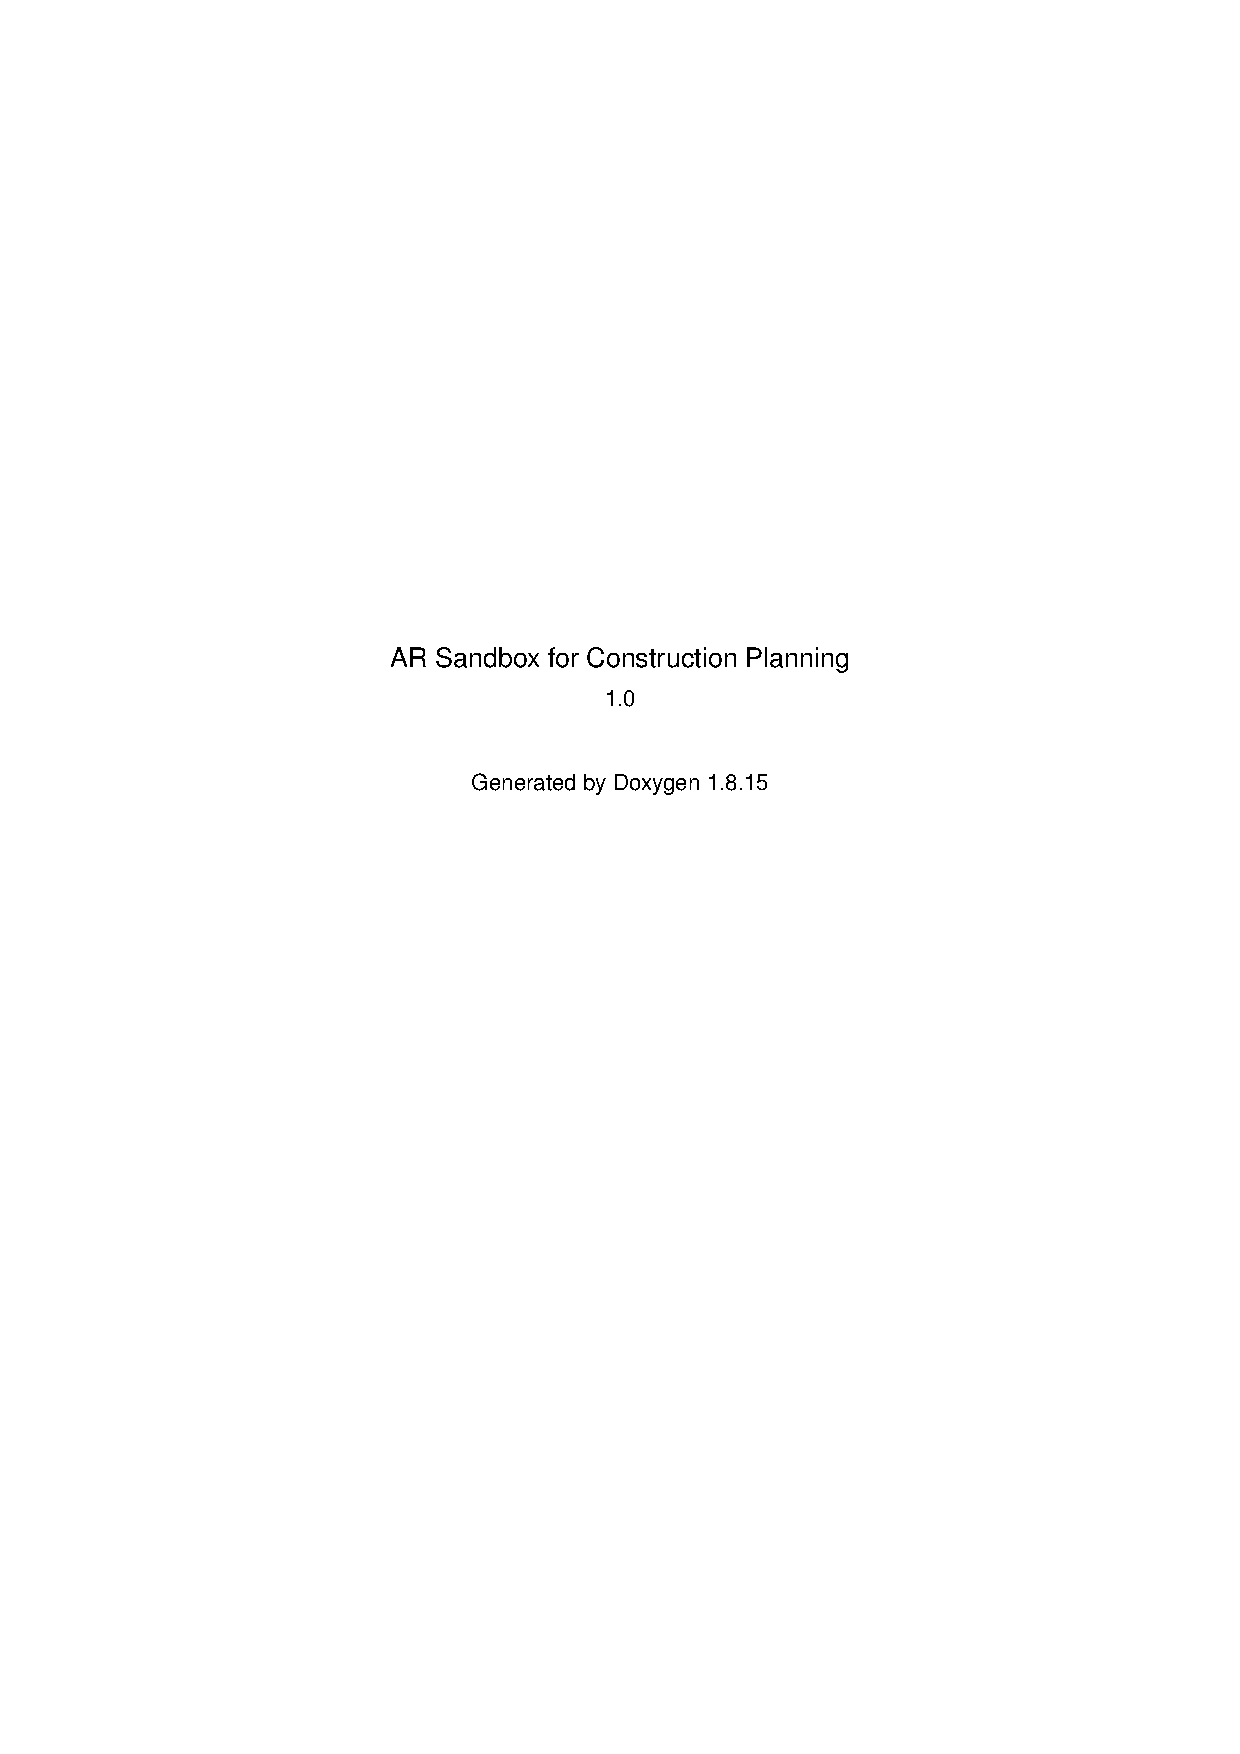
\includepdf[pages=1]{doc/refman.pdf}
    \includepdf[pages=3]{doc/refman.pdf}
    \includepdf[pages=5]{doc/refman.pdf}

%SECTION APPENDICES
\newpage
\appendices

%SECTION REFS
\newpage
\nocite{*}
\bibliographystyle{IEEEtran}
\bibliography{references}
        
\end{document}